\documentclass[../main.tex]{subfiles}

\begin{document}
Dựa vào sự phát triển và đặc điểm của dịch bệnh COVID-19, ta sẽ sử dụng mô hình SEIR để nghiên cứu sự lan truyền của dịch. Giả sử rằng $N$ là kích cỡ dân số của Trung Quốc (xấp xỉ 1,4 tỷ người). Tập dân số sẽ được chia thành các nhóm rời rạc như mẫn cảm $S(t)$, phơi nhiễm $E(t)$, nhiễm bệnh $I(t)$, điều trị $H(t)$, phục hồi $R(t)$. Các trường hợp tiếp xúc với người bệnh được tìm thấy sẽ được cách ly và theo dõi là $S_q(t)$ và $E_q(t)$. Trong đó, $S_q(t)$ là những người không bị nhiễm bệnh và sẽ được thả về sau thời gian cách ly; $E_q(t)$ là những người sẽ bị nhiễm bệnh trong thời gian cách ly. Ở đây, biến $t$ là biến thời gian rời rạc để miêu tả sự tiếp triển của dịch bệnh qua từng ngày. Bước thời gian là một ngày $h=1$. Tại một thời điểm, số lượng cá thể của mỗi nhóm sẽ phụ thuốc vào số lượng của ngày hôm trước và sự thay đổi giữa các nhóm của ngày hôm đó. Đặt $B_{ij}(t)$ là số lượng các cá thể dịch chuyển giữa các nhóm. Ta định nghĩa chi tiết như sau:
\begin{itemize}
    \item $B_{11}(t)$ là số người mới bị mắc bệnh đang trong thời gian ủ bệnh
    \item $B_{12}(t)$ là số người bị cách ly do tiếp xúc với người bệnh những không bị nhiễm
    \item $B_{21}(t)$ là số người bị mắc bệnh với các triệu chứng rõ ràng
    \item $B_{31}(t)$ là số người được xác minh nhiễm bệnh và được đưa vào điều trị
    \item $B_{32}(t)$ là số ca tử vong từ những người bị nhiễm bệnh (chưa qua điều trị)
    \item $B_{33}(t)$ là số người bị bệnh nhưng có khả năng tự phục hồi
    \item $B_{41}(t)$ là số người đã hoàn thành cách ly và được thả về
    \item $B_{51}(t)$ là số người được đưa vào điều trị từ khu cách ly
    \item $B_{61}(t)$ là số người phục hồi sau quá trình điều trị
    \item $B_{61}(t)$ là số ca tử vong trong quá trình điều trị
\end{itemize}
Sự dịch chuyển của một người từ nhóm này sang nhóm kia được coi là một quá trình ngẫu nhiên. Khoảng thời gian một người ở trong một nhóm nhất định được coi là tuân theo phân phối mũ. Nếu ta giả sử rằng tham số của phân phối mũ là $\lambda (t)$, thì xác suất rời khỏi nhóm hiện tại trong khoảng thời gian $h$ là $1-exp(-\lambda (t)h)$. Mặt khác, số lượng dòng vào và ra của một trạng thái hay là $B_{ij}(t)$ được cho là tuân theo phân phối nhị thức $Bin(n,p)$. Trong đó $n$ bằng số lượng người trong nhóm hiện tại. Sự lan truyền của dịch bệnh được được diễn ra thông qua tiếp xúc với người bệnh. Giả sử xác suất lan truyền là $\beta$ và tỷ lệ tiếp xúc là $c(t)$ thì $\beta c(t) I(t) / N$ là tham số của phân phối mũ của xác suất các cá thể có thể bị nhiễm bệnh khi tiếp xúc với người bệnh. Giả sử $q$ là tỷ lệ những trường hợp nhiễm bệnh bị cách ly. Dựa vào những giả định trên và mô hình SEIR đã được phát triển \cite{seir}, ta có mô hình như sau:
\begin{align*}
    & S(t+h)=S(t)-B_{11}(t)-B_{12}(t)+B_{41}(t) \\
    & E(t+h)=E(t)+(1-q)B_{11}(t)-B_{21}(t) \\
    & I(t+h)=I(t)+B_{21}(t)-B_{31}(t)-B_{32}(t)-B_{33}(t) \\
    & S_q(t+h)=S_q(t)+B_{12}(t)-B_{41}(t) \\
    & E_q(t+h)=E_q(t)+qB_{11}(t)-B_{51}(t) \\
    & H(t+h)=H(t)+B_{31}(t)+B_{51}(t)-B_{61}(t)-B_{62}(t) \\
    & R(t+h)=R(t)+B_{33}(t)+B_{61}(t)
\end{align*}
trong đó
\begin{align*}
    & B_{11}(t) \sim Poi(S(t)*P_{11}(t)), \quad B_{12}(t) \sim Poi(S(t)*P_{12}(t)), \\
    & B_{21}(t) \sim Bin(E(t),P_{21}), \quad B_{31}(t) \sim Bin(I(t),P_{31}), \\
    & B_{32}(t) \sim Bin(I(t),P_{32}), \quad B_{33}(t) \sim Bin(I(t),P_{33}), \\
    & B_{41}(t) \sim Bin(S_q(t),P_{41}), \quad B_{51}(t) \sim Bin(E_q(t),P_{51}), \\
    & B_{61}(t) \sim Bin(H(t),P_{61}), \quad B_{62}(t) \sim Bin(H(t),P_{32})
\end{align*}
Các xác suất trong các phân phối nhị thức trên được mô tả chi tiết như sau:
\begin{align*}
    & P_{11}(t)=1-exp(-\beta c(t) I(t)h/N), \quad P_{12}(t)=1-exp(-c(t)q(1-\beta)I(t)h/N), \\
    & P_{21}=1-exp(-\sigma h), \quad P_{31}=1-exp(-\delta _I h), \\
    & P_{32}=1-exp(-\alpha h), \quad P_{33}=1-exp(-\gamma _I h), \\
    & P_{41}=1-exp(-\lambda h), \quad P_{51}=1-exp(-\delta _q h), P_{61}=1-exp(-\gamma _H h)
\end{align*}

Lưu ý rằng số lượng người ở $S(t)$ xấp xỉ bằng tổng dân số $N$ ở Trung Quốc. Do giới hạn của phân phối nhị thức là phân phối Poisson và số lượng người ở $S(t)$ là lớn. Vì vậy mà $B_{11}(t)$ và $B_{12}(t)$ tuân theo phân phối Poisson. Tổng quát của mô hình được miêu tả bằng biểu đồ \ref{diagram}. Các tham số của mô hình được tổng kết ở bảng 1.
\begin{figure}[H]
\centering
\resizebox{15cm}{!}{
\tikzset{every picture/.style={line width=0.75pt}} %set default line width to 0.75pt        

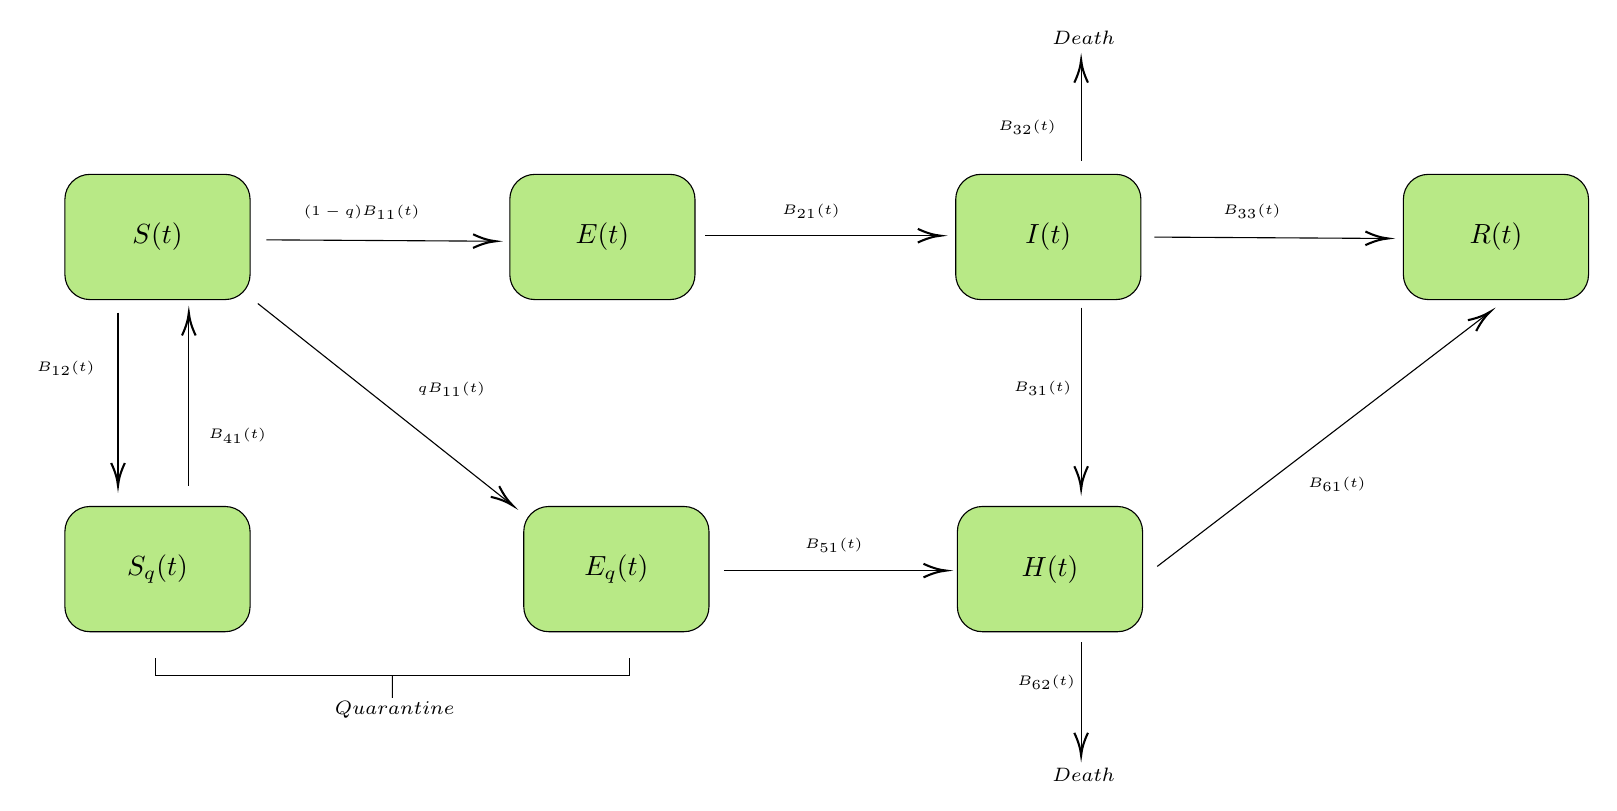
\begin{tikzpicture}[x=0.75pt,y=0.75pt,yscale=-1,xscale=1]
%uncomment if require: \path (0,470); %set diagram left start at 0, and has height of 470

%Rounded Rect [id:dp7623246854359582] 
\draw  [fill={rgb, 255:red, 184; green, 233; blue, 134 }  ,fill opacity=1 ] (85.13,139.47) .. controls (85.13,132.8) and (90.53,127.4) .. (97.19,127.4) -- (162.28,127.4) .. controls (168.95,127.4) and (174.35,132.8) .. (174.35,139.47) -- (174.35,175.67) .. controls (174.35,182.34) and (168.95,187.74) .. (162.28,187.74) -- (97.19,187.74) .. controls (90.53,187.74) and (85.13,182.34) .. (85.13,175.67) -- cycle ;
%Rounded Rect [id:dp4768493132481155] 
\draw  [fill={rgb, 255:red, 184; green, 233; blue, 134 }  ,fill opacity=1 ] (85.13,299.49) .. controls (85.13,292.82) and (90.53,287.42) .. (97.19,287.42) -- (162.28,287.42) .. controls (168.95,287.42) and (174.35,292.82) .. (174.35,299.49) -- (174.35,335.69) .. controls (174.35,342.36) and (168.95,347.76) .. (162.28,347.76) -- (97.19,347.76) .. controls (90.53,347.76) and (85.13,342.36) .. (85.13,335.69) -- cycle ;

%Rounded Rect [id:dp3654569066911406] 
\draw  [fill={rgb, 255:red, 184; green, 233; blue, 134 }  ,fill opacity=1 ] (299.49,139.47) .. controls (299.49,132.8) and (304.89,127.4) .. (311.55,127.4) -- (376.64,127.4) .. controls (383.31,127.4) and (388.71,132.8) .. (388.71,139.47) -- (388.71,175.67) .. controls (388.71,182.34) and (383.31,187.74) .. (376.64,187.74) -- (311.55,187.74) .. controls (304.89,187.74) and (299.49,182.34) .. (299.49,175.67) -- cycle ;

%Rounded Rect [id:dp5762944212255994] 
\draw  [fill={rgb, 255:red, 184; green, 233; blue, 134 }  ,fill opacity=1 ] (306.22,299.49) .. controls (306.22,292.82) and (311.63,287.42) .. (318.29,287.42) -- (383.38,287.42) .. controls (390.05,287.42) and (395.45,292.82) .. (395.45,299.49) -- (395.45,335.69) .. controls (395.45,342.36) and (390.05,347.76) .. (383.38,347.76) -- (318.29,347.76) .. controls (311.63,347.76) and (306.22,342.36) .. (306.22,335.69) -- cycle ;

%Rounded Rect [id:dp021595159630125815] 
\draw  [fill={rgb, 255:red, 184; green, 233; blue, 134 }  ,fill opacity=1 ] (514.33,139.47) .. controls (514.33,132.8) and (519.74,127.4) .. (526.4,127.4) -- (591.49,127.4) .. controls (598.16,127.4) and (603.56,132.8) .. (603.56,139.47) -- (603.56,175.67) .. controls (603.56,182.34) and (598.16,187.74) .. (591.49,187.74) -- (526.4,187.74) .. controls (519.74,187.74) and (514.33,182.34) .. (514.33,175.67) -- cycle ;

%Rounded Rect [id:dp8968884149325778] 
\draw  [fill={rgb, 255:red, 184; green, 233; blue, 134 }  ,fill opacity=1 ] (515.13,299.49) .. controls (515.13,292.82) and (520.53,287.42) .. (527.19,287.42) -- (592.28,287.42) .. controls (598.95,287.42) and (604.35,292.82) .. (604.35,299.49) -- (604.35,335.69) .. controls (604.35,342.36) and (598.95,347.76) .. (592.28,347.76) -- (527.19,347.76) .. controls (520.53,347.76) and (515.13,342.36) .. (515.13,335.69) -- cycle ;

%Rounded Rect [id:dp4560508594384034] 
\draw  [fill={rgb, 255:red, 184; green, 233; blue, 134 }  ,fill opacity=1 ] (730,139.47) .. controls (730,132.8) and (735.4,127.4) .. (742.07,127.4) -- (807.15,127.4) .. controls (813.82,127.4) and (819.22,132.8) .. (819.22,139.47) -- (819.22,175.67) .. controls (819.22,182.34) and (813.82,187.74) .. (807.15,187.74) -- (742.07,187.74) .. controls (735.4,187.74) and (730,182.34) .. (730,175.67) -- cycle ;
%Straight Lines [id:da9482455901186368] 
\draw    (110.72,194.08) -- (110.72,275.42) ;
\draw [shift={(110.72,277.42)}, rotate = 270] [color={rgb, 255:red, 0; green, 0; blue, 0 }  ][line width=0.75]    (10.93,-3.29) .. controls (6.95,-1.4) and (3.31,-0.3) .. (0,0) .. controls (3.31,0.3) and (6.95,1.4) .. (10.93,3.29)   ;
%Straight Lines [id:da05728303880138008] 
\draw    (144.84,277.42) -- (144.84,196.08) ;
\draw [shift={(144.84,194.08)}, rotate = 450] [color={rgb, 255:red, 0; green, 0; blue, 0 }  ][line width=0.75]    (10.93,-3.29) .. controls (6.95,-1.4) and (3.31,-0.3) .. (0,0) .. controls (3.31,0.3) and (6.95,1.4) .. (10.93,3.29)   ;
%Straight Lines [id:da4884708529781723] 
\draw    (357.14,360.65) -- (357.14,368.99) -- (128.72,368.99) -- (128.72,360.6) ;
%Straight Lines [id:da10074852907910814] 
\draw    (242.91,379.65) -- (242.93,368.99) ;
%Straight Lines [id:da11296625559642659] 
\draw    (182.18,158.96) -- (290.73,159.61) ;
\draw [shift={(292.73,159.63)}, rotate = 180.35] [color={rgb, 255:red, 0; green, 0; blue, 0 }  ][line width=0.75]    (10.93,-3.29) .. controls (6.95,-1.4) and (3.31,-0.3) .. (0,0) .. controls (3.31,0.3) and (6.95,1.4) .. (10.93,3.29)   ;
%Straight Lines [id:da37586070655180936] 
\draw    (178.08,189.63) -- (299.35,285.73) ;
\draw [shift={(300.92,286.98)}, rotate = 218.4] [color={rgb, 255:red, 0; green, 0; blue, 0 }  ][line width=0.75]    (10.93,-3.29) .. controls (6.95,-1.4) and (3.31,-0.3) .. (0,0) .. controls (3.31,0.3) and (6.95,1.4) .. (10.93,3.29)   ;
%Straight Lines [id:da7761382576789853] 
\draw    (402.6,318.31) -- (507.73,318.31) ;
\draw [shift={(509.73,318.31)}, rotate = 180] [color={rgb, 255:red, 0; green, 0; blue, 0 }  ][line width=0.75]    (10.93,-3.29) .. controls (6.95,-1.4) and (3.31,-0.3) .. (0,0) .. controls (3.31,0.3) and (6.95,1.4) .. (10.93,3.29)   ;
%Straight Lines [id:da9729894086577398] 
\draw    (393.72,156.96) -- (505,156.96) ;
\draw [shift={(507,156.96)}, rotate = 180] [color={rgb, 255:red, 0; green, 0; blue, 0 }  ][line width=0.75]    (10.93,-3.29) .. controls (6.95,-1.4) and (3.31,-0.3) .. (0,0) .. controls (3.31,0.3) and (6.95,1.4) .. (10.93,3.29)   ;
%Straight Lines [id:da45085066783261496] 
\draw    (574.75,191.63) -- (574.75,276.97) ;
\draw [shift={(574.75,278.97)}, rotate = 270] [color={rgb, 255:red, 0; green, 0; blue, 0 }  ][line width=0.75]    (10.93,-3.29) .. controls (6.95,-1.4) and (3.31,-0.3) .. (0,0) .. controls (3.31,0.3) and (6.95,1.4) .. (10.93,3.29)   ;
%Straight Lines [id:da5455110861418122] 
\draw    (574.75,120.95) -- (574.75,74.28) ;
\draw [shift={(574.75,72.28)}, rotate = 450] [color={rgb, 255:red, 0; green, 0; blue, 0 }  ][line width=0.75]    (10.93,-3.29) .. controls (6.95,-1.4) and (3.31,-0.3) .. (0,0) .. controls (3.31,0.3) and (6.95,1.4) .. (10.93,3.29)   ;
%Straight Lines [id:da20700401454618644] 
\draw    (574.75,352.73) -- (574.75,405.41) ;
\draw [shift={(574.75,407.41)}, rotate = 270] [color={rgb, 255:red, 0; green, 0; blue, 0 }  ][line width=0.75]    (10.93,-3.29) .. controls (6.95,-1.4) and (3.31,-0.3) .. (0,0) .. controls (3.31,0.3) and (6.95,1.4) .. (10.93,3.29)   ;
%Straight Lines [id:da049411173786683804] 
\draw    (611.41,316.31) -- (770.19,194.85) ;
\draw [shift={(771.78,193.63)}, rotate = 502.58] [color={rgb, 255:red, 0; green, 0; blue, 0 }  ][line width=0.75]    (10.93,-3.29) .. controls (6.95,-1.4) and (3.31,-0.3) .. (0,0) .. controls (3.31,0.3) and (6.95,1.4) .. (10.93,3.29)   ;
%Straight Lines [id:da5803439064982177] 
\draw    (610.05,157.63) -- (720.64,158.28) ;
\draw [shift={(722.64,158.29)}, rotate = 180.34] [color={rgb, 255:red, 0; green, 0; blue, 0 }  ][line width=0.75]    (10.93,-3.29) .. controls (6.95,-1.4) and (3.31,-0.3) .. (0,0) .. controls (3.31,0.3) and (6.95,1.4) .. (10.93,3.29)   ;

% Text Node
\draw (129.74,157.57) node   [align=left] {$\displaystyle S( t)$};
% Text Node
\draw (774.61,157.57) node   [align=left] {$\displaystyle R( t)$};
% Text Node
\draw (129.74,317.59) node   [align=left] {$\displaystyle S_{q}( t)$};
% Text Node
\draw (344.1,157.57) node   [align=left] {$\displaystyle E( t)$};
% Text Node
\draw (350.84,317.59) node   [align=left] {$\displaystyle E_{q}( t)$};
% Text Node
\draw (559.74,317.59) node   [align=left] {$\displaystyle H( t)$};
% Text Node
\draw (558.95,157.57) node   [align=left] {$\displaystyle I( t)$};
% Text Node
\draw (228.13,145.62) node  [font=\tiny] [align=left] {$\displaystyle ( 1-q) B_{11}( t)$};
% Text Node
\draw (271.34,230.89) node  [font=\tiny] [align=left] {$\displaystyle qB_{11}( t)$};
% Text Node
\draw (85.46,220.88) node  [font=\tiny] [align=left] {$\displaystyle B_{12}( t)$};
% Text Node
\draw (168.2,253.39) node  [font=\tiny] [align=left] {$\displaystyle B_{41}( t)$};
% Text Node
\draw (213.93,380) node [anchor=north west][inner sep=0.75pt]  [font=\scriptsize] [align=left] {$\displaystyle Quarantine$};
% Text Node
\draw (440.42,301.42) node [anchor=north west][inner sep=0.75pt]  [font=\tiny] [align=left] {$\displaystyle B_{51}( t)$};
% Text Node
\draw (542.78,367.26) node [anchor=north west][inner sep=0.75pt]  [font=\tiny] [align=left] {$\displaystyle B_{62}( t)$};
% Text Node
\draw (548.64,104.62) node  [font=\tiny] [align=left] {$\displaystyle B_{32}( t)$};
% Text Node
\draw (444.57,145.04) node  [font=\tiny] [align=left] {$\displaystyle B_{21}( t)$};
% Text Node
\draw (541.07,225.58) node [anchor=north west][inner sep=0.75pt]  [font=\tiny] [align=left] {$\displaystyle B_{31}( t)$};
% Text Node
\draw (656.97,145.04) node  [font=\tiny] [align=left] {$\displaystyle B_{33}( t)$};
% Text Node
\draw (697.92,276.72) node  [font=\tiny] [align=left] {$\displaystyle B_{61}( t)$};
% Text Node
\draw (559.6,57) node [anchor=north west][inner sep=0.75pt]  [font=\scriptsize] [align=left] {$\displaystyle Death$};
% Text Node
\draw (559.6,412) node [anchor=north west][inner sep=0.75pt]  [font=\scriptsize] [align=left] {$\displaystyle Death$};


\end{tikzpicture}
}
\caption{Biểu đồ dòng miêu tả sự lây nhiễm của dịch bệnh COVID-19}
\label{diagram}
\end{figure}

Hạn chế tiếp xúc là một biện pháp phòng chống dịch bệnh hiệu quả để kiểm soát sự lây lan của dịch bệnh. Nâng cao nhận thức của cộng đồng về phòng ngừa dịch bệnh và hạn chế di chuyển hoặc đeo khẩu trang khi ở nơi công cộng. Trong mô hình này, tỷ lệ tiếp xúc $c(t)$ (tức là số lượng tiếp xúc trung bình của một người trên một đơn vị thời gian) được coi là một hàm thành phần. Nó là hằng số trước thời điểm $t^*$ hay là trước thời điểm các biện pháp giãn cách xã hội được thực hiện. Ta giả định rằng nó sẽ giảm dần từ $c_0$ đến $c_u$. Khi đó ta có hàm $c(t)$:
\begin{align*}
    c(t) = 
    \begin{cases}
    c_0  & \mbox{nếu } t \leq t^* \\
    (c_0 -c_u)e^{-k(t-t^*)}+c_u & \mbox{nếu } t > t^*
    \end{cases}
\end{align*}
Các biện pháp cách ly được áp dụng ở Trung Quốc từ ngày 23 tháng 1 năm 2020. Dữ liệu được thu thập từ ngày 11 tháng 1 năm 2020. Do đó, $t^*=12$.
\begin{figure}[H]
    \centering
    \caption*{\textbf{Bảng 1:} các tham số đã được ước lượng và ban đầu của mô hình}
    \resizebox{15cm}{!}{\renewcommand{\arraystretch}{1.25}
\begin{tabular}{l p{5.5cm} l l l l l}
\hline 
 Parameters & Definition & Baseline values & Range & Means value & (estimated)Std & Source \\
\hline 
 $\displaystyle c_{0}$ & Tỷ lệ tiếp xúc ban đầu & $\displaystyle 31$ & $\displaystyle ( 0,50]$ & $\displaystyle 34.037$ & $\displaystyle 0.389$ & $\displaystyle MCMC$ \\
$\displaystyle c_{u}$ & Tỷ lệ tiếp xúc thấp nhất khi đã áp dụng các biện pháp giãn cách xã hội & $\displaystyle 1$ & $\displaystyle ( 0,50]$ & $\displaystyle 0.933$ & $\displaystyle 0.0037$ & $\displaystyle MCMC$ \\
$\displaystyle k$ & Tỷ lệ giảm của tỷ lệ tiếp xúc theo thời gian & $\displaystyle 0.1$ & $\displaystyle [ 0,1]$ & $\displaystyle 0.144$ & $\displaystyle 0.0035$ & $\displaystyle MCMC$ \\
$\displaystyle \beta $ & Xác suất lan truyền của dịch bệnh & $\displaystyle 0.095$ & $\displaystyle [ 0,1]$ & $\displaystyle 0.111$ & $\displaystyle 0.0015$ & $\displaystyle MCMC$ \\
$\displaystyle q$ & Tỷ lệ cách ly những trường hợp bị phơi nhiễm & $\displaystyle 0.4$ & $\displaystyle [ 0,1]$ & $\displaystyle 0.415$ & $\displaystyle 0.016$ & $\displaystyle MCMC$ \\
$\displaystyle \sigma $ & Tỷ lệ chuyển từ trạng thái $E$ sang $I$ & $\displaystyle 1/7$ & $\displaystyle [ 0,1]$ & $\displaystyle 1/7$ & $\displaystyle \_$ & \cite{ncovid} \\
$\displaystyle \lambda $ & Tỷ lệ chuyển từ $S_q$ sang $S$ (được thả từ cách ly) & $\displaystyle 1/14$ & $\displaystyle [ 0,1]$ & $\displaystyle 1/14$ & $\displaystyle \_$ & \cite{ncovid} \\
$\displaystyle \delta _{I}$ & Tỷ lệ chuyển từ $I$ sang $H$ & $\displaystyle 0.1$ & $\displaystyle [ 0,1]$ & $\displaystyle 0.304$ & $\displaystyle 0.001$ & $\displaystyle MCMC$ \\
$\displaystyle \delta _{q}$ & Tỷ lệ chuyển từ $E_q$ sang $H$ & $\displaystyle 0.42$ & $\displaystyle [ 0,1]$ & $\displaystyle 0.413$ & $\displaystyle 0.0116$ & $\displaystyle MCMC$ \\
$\displaystyle \gamma _{I}$ & Tỷ lệ chuyển từ $I$ sang $R$ (tỷ lệ những trường hợp có khả năng tự hồi phục) & $\displaystyle 0.008$ & $\displaystyle [ 0,1]$ & $\displaystyle 0.0085$ & $\displaystyle 0.0001$ & $\displaystyle MCMC$ \\
$\displaystyle \gamma _{H}$ & Tỷ lệ chuyển từ $H$ sang $R$ (tỷ lệ hồi phục sau khi được chăm sóc y tế) & $\displaystyle 0.017$ & $\displaystyle [ 0,1]$ & $\displaystyle 0.018$ & $\displaystyle 0.0003$ & $\displaystyle MCMC$ \\
$\displaystyle \alpha $ & Tỷ lệ chết & $\displaystyle 0.0027$ & $\displaystyle [ 0,1]$ & $\displaystyle 0.0027$ & $\displaystyle 0.0001$ & $\displaystyle MCMC$ \\
\hline 
 $\displaystyle N$ & Toàn bộ dân số (xấp xỉ S) & $\displaystyle \_$ & $\displaystyle \_$ & $\displaystyle 1.4\times 14^{10}$ & $\displaystyle \_$ & $\displaystyle Data$ \\
$\displaystyle E( 0)$ & Các trường hợp phơi nhiễm ban đầu & $\displaystyle 105$ & $\displaystyle [ 1,200]$ & $\displaystyle 52$ & $\displaystyle 0.64$ & $\displaystyle MCMC$ \\
$\displaystyle I( 0)$ & Các trường hợp nhiễm bệnh ban đầu & $\displaystyle 54$ & $\displaystyle [ 1,100]$ & $\displaystyle 31$ & $\displaystyle 0.346$ & $\displaystyle MCMC$ \\
$\displaystyle S_{q}( 0)$ & Các trường hợp không bị phơi nhiễm được cách ly ban đầu & $\displaystyle \_$ & $\displaystyle \_$ & $\displaystyle 734$ & $\displaystyle \_$ & $\displaystyle Data$ \\
$\displaystyle E_{q}( 0)$ & Các trường hợp bị phơi nhiễm được cách ly ban đầu & $\displaystyle 2$ & $\displaystyle [ 0,100]$ & $\displaystyle 5$ & $\displaystyle 0.24$ & $\displaystyle MCMC$ \\
$\displaystyle H( 0)$ & Các trường hợp nhiễm bệnh được chăm sóc y tế ban đầu  & $\displaystyle \_$ & $\displaystyle \_$ & $\displaystyle 41$ & $\displaystyle \_$ & $\displaystyle Data$ \\
$\displaystyle R( 0)$ & Các trường hợp hồi phục ban đầu & $\displaystyle \_$ & $\displaystyle \_$ & $\displaystyle 6$ & $\displaystyle \_$ & $\displaystyle Data$ \\
\hline
\end{tabular}}
    \label{table:1}
\end{figure}
\end{document}